\section{Aplikacje okienkowe - {\tt System.Windows.Forms}}

Jak widzieliśmy w poprzednich rozdziałach, programowanie Windows nie polega wyłącznie na tworzeniu okien,
jednak z pewnością to właśnie temu zagadnieniu programista poświęca zwykle sporo czasu. 
Od dobrej biblioteki wspierającej tworzenie okien i własnych komponentów należałoby oczekiwać prostoty
i spójności. Z perspektywy historycznej można powiedzieć, że Win32Api jest interfejsem spójnym jednak dość
żmudnym. W kolejnych latach powstawały więc kolejne wyspecjalizowane bibilioteki, 
wspierające tworzenie aplikacji okienkowych. Dużą populaność zdobył sobie również Visual Basic, 
w którym projektowanie interfejsu użytkownika było wyjątkowo proste, jednak interfejs programowania
był bardzo niespójny - często podobne czynności w różnych kontekstach realizowane były za pomocą
zupełnie różnych mechanizmów\footnote{Visual Basic z czasów przed VB.NET jest również dość słaby jako
język programowania, ponieważ ma ubogi i nieprzemyślany model obiektowy.}. 

Biblioteka {\bf System.Windows.Forms}, która umożliwia tworzenie aplikacji okienkowych w świecie .NET
jest zarówno prosta jak i spójna. Nie sprawi kłopotu ani nowicjuszowi, który chciałby nauczyć się 
tworzyć okna jak najszybciej, ani profesjonaliście, który znając ułomności innych interfejsów szybko
nauczy się korzystać z zaawansowanych mechanizmów biblioteki {\em System.Windows.Forms}. Tworzenie
interfejsu użytkownika jest równie proste jak w "starym" Visual Basicu, zaś kontrola, jaką programista
ma nad oprogramowywanym interfejsem, dorównuje tej, jaką daje Win32Api.

{\bf System.Windows.Forms}, jako interfejs w pełni obiektowy, najbardziej przypomina biblioteki
okienkowe Javy. Dla programisty najważniejsze jest to, że cały opis komponentu (okna, kontrolki) jest
częścią kodu, dzięki czemu kod nie jest w żaden sposób związany z jakimś środowiskiem developerskim.
Przy odrobinie wprawy można z powodzeniem pisać programy okienkowe używając dowolnego edytora tekstu,
nawet zwykłego Notatnika.

Interfejs obiekty oznacza również, że funkcjonalność każdego komponentu można bardzo łatwo rozszerzyć
tworząc w razie potrzeby klasę potomną dziedziczącą z niego. Programista może również w łatwy sposób
tworzyć własne komponenty wizualne (kontrolki), do których może zaprojektować własne zdarzenia. 

\subsection{Tworzenie okien}
\label{netTworzenieOkien}

Przypomnijmy sobie najprostszy program ze strony \pageref{tworzenieOkienAPI}, który tworzył zwykłe, 
proste okno na pulpicie. Jego odpowiednik w świecie .NET wygląda tak:

\begin{scriptsize}
\begin{verbatim}
/* Wiktor Zychla, 2003 */
using System;
using System.Windows.Forms;

namespace Example
{
  public class CMainForm : Form
  {   
    public CMainForm()
    {
      this.Text = "Okna w świecie .NET"; 
    }

    public static void Main()
    {
      Application.Run( new CMainForm() );
    }
  }
}
\end{verbatim}
\end{scriptsize}

Różnica w przejrzystości programu jest kolosalna! Interfejs biblioteki {\bf System.Windows.Forms} jest
w pełni obiektowy. Utworzenie okna polega po prostu na utworzeniu klasy dziedziczącej z klasy
{\bf Form}. Klasa ta zamyka w sobie całą funkcjonalność jakiej potrzeba aby obsłużyć proste okno: obiekt
który utworzyliśmy w przykładowym programie powyżej ma kilkadziesiąt propercji i metod oraz obsługuje
kilkadziesiąt zdarzeń.

Powyższy kod może w pierwszej chwili wydawać się dość zaskakujący, bowiem nie ma tu nigdzie
pętli obsługi komunikatów. Okazuje się, że pętla obsługi komunikatów jest ukryta w funkcji
{\bf Run} klasy {\bf Application}. Dodatkowym, opcjonalnym parametrem metody {\bf Run} jest
obiekt, będący {\em głównym oknem aplikacji}. Aplikacja automatycznie zakończy się, kiedy główne
okno aplikacji zostanie zniszczone.

Oczywiście taka konstrukcja utrudnia nieco sterowanie aplikacją wtedy, gdy powinna ona
zajmować się czymś oprócz przetwarzania komunikatów. 
Na stronie \pageref{apiPetlaObslugiKomunikatow} widzieliśmy jak radzić sobie z takim problemem w Win32Api
(zamiast {\bf GetMessage} użyliśmy {\bf PeekMessage}),
zaś na stronie \pageref{netPetlaObslugiKomunikatow} pokazano jak wygląda analogiczna konstrukcja
w świecie .NET.

Widać również, że programista w przeciwieństwie do Win32API nie musi samodzielnie 
rejestrować klasy okna w systemie. Właściwości klasy okna opisuje definicja klasy, zaś sama operacja
rejestrowania klasy okna w systemie odbywa się bez udziału programisty\footnote{W świecie
.NET definicja okna jest klasą. Aby takie okno mogło pojawić się w systemie, w systemie rejestrowana jest
oczywiście klasa okna. Nie należy jednak mylić tych dwóch pojęć i dlatego wprowadzimy dwa różne określenia:
{\em klasą okna} będziemy nazywać obiekt systemowy, opisujący właściwości okna i rejestrowany w systemie
za pomocą funkcji {\bf RegisterClass}, zaś {\em klasą opisującą okno}, będziemy nazywać definicję
klasy dziedziczącej z klasy {\bf Form}, opisującej właściwości okna w C\#.}.

\subsection{Okna potomne}

W obiektowym świecie {\bf System.Windows.Forms}, każdy obiekt dziedziczący z klasy {\bf Control} (klasa
{\bf Form} dziedziczy z klasy {\bf Control} i jest od niej odległa o 4 pokolenia) ma propercję
{\bf Controls}, która zwraca kolekcję okien potomnych względem tego obiektu. Oznacza to, że
okna potomne mogą być łatwo tworzone w czasie działania programu. Te okna potomne, które powinny
być widoczne od razu po utworzeniu okna można utworzyć po prostu w konstruktorze okna macierzystego.

Najwygodniej jest uczynić okna potomne polami składowymi klasy opisującej okno macierzyste. Wtedy wszystkie
inne składowe klasy okna macierzystego mają dostęp do okien potomnych. Okna potomne są również obiektami,
podlegają więc dokładnie takim samym prawom jak wszystkie obiekty - muszą być jawnie
skonstruowane, są odśmiecane itd.

\begin{figure}
\begin{center}
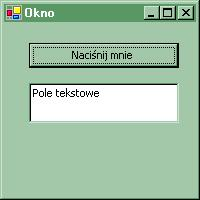
\includegraphics[width=0.30\textwidth]{./pic/n01}
\caption{Proste okno w świecie .NET}
\end{center}
\end{figure}

\begin{scriptsize}
\begin{verbatim}
/* Wiktor Zychla, 2003 */
using System;
using System.Drawing;
using System.Windows.Forms;

namespace Example
{
  public class CMainForm : Form
  {   
    Button  btOK;
    TextBox pTxt;   

    public CMainForm()
    {
      btOK           = new Button();     
      btOK.Location  = new Point( 25, 20 );
      btOK.Size      = new Size( 150, 25 );
      btOK.Text      = "Naciśnij mnie";

      pTxt           = new TextBox();
      pTxt.Location  = new Point( 25, 60 );
      pTxt.Size      = new Size( 150, 40 );
      pTxt.Multiline = true;
      pTxt.Text      = "Pole tekstowe";

      this.Controls.AddRange( new Control[] { btOK, pTxt } );

      this.Text = "Okno"; 
      this.Size = new Size( 200, 200 );
    }

    public static void Main()
    {
       Application.Run( new CMainForm() );
    }
  }
}
\end{verbatim}
\end{scriptsize}

Tworząc okna można zejść aż na poziom równy funkcji {\bf CreateWindow}, na którym można utworzyć
okno podając nazwę klasy okna, jego styl i rozmiary.

\begin{scriptsize}
\begin{verbatim}
/* Wiktor Zychla, 2003 */
using System;
using System.Drawing;
using System.Windows.Forms;

namespace Example
{
  public class CMainForm : Form
  {   
    const int WS_VISIBLE = 0x10000000;
    const int WS_CHILD   = 0x40000000;

    public CMainForm()
    {
      CreateParams cp = new CreateParams();
      cp.ClassName  = "EDIT";      
      cp.Style      = WS_CHILD | WS_VISIBLE;
      cp.Parent     = this.Handle;
      cp.Width      = 150;
      cp.Height     = 25;
      cp.X          = 20;
      cp.Y          = 20; 

      NativeWindow t = new NativeWindow();
      t.CreateHandle( cp );

      this.Text = "Okno"; 
      this.Size = new Size( 200, 200 );      
    }

    public static void Main()
    {
       Application.Run( new CMainForm() );
    }
  }
}
\end{verbatim}
\end{scriptsize}

\subsection{Zdarzenia}

W rozdziale \ref{delegaciZdarzenia} na stronie \pageref{delegaciZdarzenia} widzieliśmy w jaki sposób
C\# rozwiązuje problem zdarzeń. Dzięki temu, że zdarzenie jest tak naprawdę listą odpowiednich delegatów,
zajście zdarzenia może śledzić dowolna ilość słuchaczy.

Taki model doskonale sprawda się w aplikacjach okienkowych, gdzie tak naprawdę istotne są
właśnie reakcje na zdarzenia zgłaszane do okien aplikacji. Aby okna reagowały na działania użytkownika, wystarczy 
więc pod odpowiednie zdarzenia "przypiąć"ich słuchaczy. Zdarzenia udostępniane przez komponenty wizualne
dość dobrze odpowiadają komunikatom, jakie komponenty te mogłyby obsługiwać. 

\begin{scriptsize}
\begin{verbatim}
/* Wiktor Zychla, 2003 */
using System;
using System.Drawing;
using System.Windows.Forms;

namespace Example
{
  public class CMainForm : Form
  {   
    Button  btOK;
    TextBox pTxt;   

    public CMainForm()
    {
      btOK           = new Button();     
      btOK.Location  = new Point( 25, 20 );
      btOK.Size      = new Size( 150, 25 );
      btOK.Text      = "Naciśnij mnie";

      pTxt           = new TextBox();
      pTxt.Location  = new Point( 25, 60 );
      pTxt.Size      = new Size( 150, 40 );
      pTxt.Multiline = true;
      pTxt.Text      = "Pole tekstowe";

      // dodaj zdarzenia
      btOK.Click    += new EventHandler( btOk_Click );
      pTxt.KeyPress += new KeyPressEventHandler( pTxt_KeyPress );

      this.Controls.AddRange( new Control[] { btOK, pTxt } );

      this.Text = "Okno"; 
      this.Size = new Size( 200, 200 );
    }

    void btOk_Click( object sender, EventArgs e )
    {
      MessageBox.Show( "Kliknięto przycisk" ); 
    }

    void pTxt_KeyPress( object sender, KeyPressEventArgs e )
    {
      this.Text = e.KeyChar.ToString();
    }

    public static void Main()
    {
       Application.Run( new CMainForm() );
    }
  }
}
\end{verbatim}
\end{scriptsize}

Wśród ważniejszych zdarzeń warto wymienić:
\begin{itemize}
\item Click
\item DoubleClick
\item Enter
\item KeyDown
\item KeyPress
\item KeyUp
\item Leave
\item MouseDown
\item MouseHover
\item MouseUp
\item Move
\item Paint
\item Resize
\item Validating
\item Validated
\end{itemize}

\subsubsection{Parametry zdarzeń}

Przy tak dużej ilości zdarzeń pojawiają się różne problemy. Na przykład - 
różne zdarzenia mogą mieć różne ilości parametrów. Informacja o naciśnięciu klawisza
powinna nieść ze sobą informację o tym klawiszu, zaś informacja o naciśnięciu przycisku myszy powinna mówić
który przycisk został naciśnięty i jaka jest pozycja wskaźnika w oknie. Ponadto, gdyby jedna i ta sama
funkcja została przypisana do obsługi różnych zdarzeń różnych komponentów, to wewnątrz funkcji obsługującej
to zdarzenie zdecydowanie powinno dać się określić ten komponent, który spowodował powstanie zdarzenia.

Na szczęście te problemy rozwiązano dość elegancko. Przyjęto konwencję, wedle której obiekt będący
źródłem zdarzenia przekazuje się zawsze jako pierwszy parametr do delegata reagującego na zajście zdarzenia,
zaś parametry zdarzenia przekazuje się w obiektach klas dziedziczących z klasy {\bf EventArgs} jako drugi
parametr tych delegatów. Na przykład zdarzenie naciśnięcia
klawisza przekazuje swoje parametry w obiekcie typu {\bf KeyPressEventArgs}, zaś zdarzenia myszy w
obiektach typu {\bf MouseEventArgs}. 

Oznacza to, że wszyscy delegaci będący słuchaczami zdarzeń związanych z obsługą komponentów wizualnych mają
bardzo podobną postać. Nazwy tych delegatów i nazwy ich parametrów odpowiadają nazwom odpowiednich zdarzeń.

\begin{scriptsize}
\begin{verbatim}
delegate void EventHandler( object sender, EventArgs e );
delegate void KeyPressEventHandler( object sender, KeyPressEventArgs e );
...
\end{verbatim}
\end{scriptsize}

\subsubsection{Pokrywanie funkcji obsługi zdarzeń}

Oprócz możliwości przypinania słuchaczy do odpowiednich zdarzeń, istnieje możliwość
przeciążenia funkcji wirtualnych dziedziczonych z klasy {\bf Control}, będących reakcjami na zdarzenia.
W tym przypadku funkcja ma już tylko jeden parametr, określający parametry zdarzenia.

\begin{scriptsize}
\begin{verbatim}
/* Wiktor Zychla, 2003 */
using System;
using System.Drawing;
using System.Windows.Forms;

namespace Example
{
  public class CMyButton : Button
  {
    protected override void OnClick( EventArgs e )
    {
      base.OnClick( e ); 
      MessageBox.Show( "Kliknięto mnie!" );
    } 
  }

  public class CMainForm : Form
  {   
    public CMainForm()
    {
      CMyButton btOK;       

      btOK           = new CMyButton();     
      btOK.Location  = new Point( 25, 20 );
      btOK.Size      = new Size( 150, 25 );
      btOK.Text      = "Naciśnij mnie";

      this.Controls.Add( btOK );

      this.Text = "Okno"; 
      this.Size = new Size( 200, 200 );
    }

    public static void Main()
    {
       Application.Run( new CMainForm() );
    }
  }
}
\end{verbatim}
\end{scriptsize}

Nic nie stoi na przeszkodzie, aby równolegle dodać funkcje reagujące na to samo zdarzenie do odpowiedniej
listy delegatów (przy okazji zwróćmy uwagę na to w jakiej kolejności wywołają się 
oba zdarzenia. Od czego to zależy?):

\begin{scriptsize}
\begin{verbatim}
/* Wiktor Zychla, 2003 */
using System;
using System.Drawing;
using System.Windows.Forms;

namespace Example
{
  public class CMyButton : Button
  {
    protected override void OnClick( EventArgs e )
    {
      base.OnClick( e ); 
      MessageBox.Show( "Kliknięto mnie!" );
    } 
  }

  public class CMainForm : Form
  {   
    public CMainForm()
    {
      CMyButton btOK;       

      btOK           = new CMyButton();     
      btOK.Location  = new Point( 25, 20 );
      btOK.Size      = new Size( 150, 25 );
      btOK.Text      = "Naciśnij mnie";

      btOK.Click += new EventHandler( btOK_Click );

      this.Controls.Add( btOK );

      this.Text = "Okno"; 
      this.Size = new Size( 200, 200 );
    }

    public void btOK_Click( object sender, EventArgs e )
    {
      MessageBox.Show( "I znów mnie kliknięto!" );
    }

    public static void Main()
    {
       Application.Run( new CMainForm() );
    }
  }
}
\end{verbatim}
\end{scriptsize}

Powstaje więc pytanie: gdzie w takim razie określać reakcje na zdarzenia, czy przeciążając odpowiednią 
funkcję czy dokładając delegata do listy słuchaczy zdarzenia?

Odpowiedź wbrew pozorom jest dość prosta: przeciążanie funkcji obsługi zdarzenia powinno stosować się tylko
tam, gdzie reakcja na zdarzenie powinna być taka sama dla {\em wszystkich} instancji tworzonego komponentu i 
w dodatku powinna być jego trwałą właściwością. Takiej funkcji nie można już bowiem odwołać. 

Jeśli zaś reakcja na zdarzenie ma być wewnętrzną sprawą jakiejś konkretnej {\em instancji} komponentu, tam
reakcja ta powinna być delegatem na liście słuchaczy zdarzenia.

\subsection{Okna dialogowe}

Skoro okna w świecie .NET są instancjami odpowiednich klas, to tworzenie nowych okien jest tak proste
jak wykreowanie nowych obiektów. Po wykreowaniu okno może być pokazane jako modalne za pomocą metody
{\bf ShowDialog} lub jako niemodalne za pomocą {\bf Show}.

\begin{scriptsize}
\begin{verbatim}
/* Wiktor Zychla, 2003 */
using System;
using System.Drawing;
using System.Windows.Forms;

namespace Example
{
  public class CSecondaryForm : Form
  {
    public CSecondaryForm()
    {
      this.Text = "Okno dialogowe";
    }
  }

  public class CMainForm : Form
  {   
    public CMainForm()
    {
      Button btOK;       

      btOK           = new Button();     
      btOK.Location  = new Point( 25, 20 );
      btOK.Size      = new Size( 150, 25 );
      btOK.Text      = "Pokaż okno dialogowe";

      btOK.Click += new EventHandler( btOK_Click );

      this.Controls.Add( btOK );

      this.Text = "Okno"; 
      this.Size = new Size( 200, 200 );
    }

    public void btOK_Click( object sender, EventArgs e )
    {
      CSecondaryForm f = new CSecondaryForm();
      f.ShowDialog(); 
    }

    public static void Main()
    {
      Application.Run( new CMainForm() );
    }
  }
}
\end{verbatim}
\end{scriptsize}

Klasa opisująca okno może mieć dowolną ilość konstruktorów, których można użyć do przekazania
parametrów nowo tworzonym oknom.


\subsection{Subclassowanie okien}

Często przechwytywanie zdarzeń nie wystarcza, a programista chciałby sięgnąć głębiej, aż na poziom
komunikatów. 

\subsubsection{Obsługa komunikatów własnych okien}

Obsługa komunikatów nie nastręcza żadnych kłopotów jeśli to programista tworzy klasę
opisującą okno. Wystarczy po prostu przeciążyć metodę {\bf WndProc}.

\begin{scriptsize}
\begin{verbatim}
/* Wiktor Zychla, 2003 */
using System;
using System.Drawing;
using System.Windows.Forms;

namespace Example
{
  public class CMainForm : Form
  {   
    const int WM_LBUTTONDBLCLK = 0x0203;

    protected override void WndProc( ref Message m )
    {
       switch ( m.Msg )
       {
         case WM_LBUTTONDBLCLK : MessageBox.Show( "Dwuklik!" ); break;
       }
       base.WndProc( ref m );
    }

    public CMainForm()
    {
      this.Text = "Okno"; 
      this.Size = new Size( 200, 200 );
    }

    public static void Main()
    {
       Application.Run( new CMainForm() );
    }
  }
}
\end{verbatim}
\end{scriptsize}

Struktura {\bf Message} przechowuje w sobie wszystkie parametry komunikatu ({\bf LParam}, {\bf WParam}, itd.),
ma również metodę {\bf GetLParam}, która służy do rzutowania parametru przekazanego w {\bf LParam} na wskazany
typ.

Warto zwrócić uwagę na konieczność wywołania funkcji {\bf WndProc} z klasy bazowej. Bez tego wywołania okno
nie utworzy się, bowiem zabraknie mu większości potrzebnej funkcjonalności.

\subsubsection{Obsługa komunikatów istniejących okien}

Przedstawiona w poprzednim podrozdziale technika nie nadaje się do obsługi komunikatów w już istniejących
komponentach, na przykład {\bf TextBox} czy {\bf Button}. Możnaby co prawda przeciążyć już istniejący komponent
i dodać obsługę komunikatów do klasy potomnej, ale interesująca byłaby możliwość taka jak opisana na stronie
\pageref{subclassingAPIFunkcje}, czyli dodawanie własnej funkcji obsługi do już istniejącego
okna.

Okazuje się, że i taki scenariusz jest możliwy, wymaga jedynie utworzenia klasy dziedziczącej z klasy
{\bf NativeWindow} i skojarzenia uchwytów okien. 

\begin{scriptsize}
\begin{verbatim}
/* Wiktor Zychla, 2003 */
using System;
using System.Drawing;
using System.Windows.Forms;

namespace Example
{
  public class CSubclass : NativeWindow
  {
    const int WM_LBUTTONDBLCLK = 0x0203;

    protected override void WndProc( ref Message m )
    {
       switch ( m.Msg )
       {
         case WM_LBUTTONDBLCLK : MessageBox.Show( "Dwuklik!" ); break;
       }
       base.WndProc( ref m );
    }

    public CSubclass() {} 
  }

  public class CMainForm : Form
  {   
    CSubclass subclass = new CSubclass();
    TextBox t;

    public CMainForm()
    {
      t = new TextBox();
      this.Controls.Add( t );

      // subclassing okna potomnego
      subclass.AssignHandle( t.Handle );

      this.Text = "Okno"; 
      this.Size = new Size( 200, 200 );      
    }

    public static void Main()
    {
       Application.Run( new CMainForm() );
    }
  }
}
\end{verbatim}
\end{scriptsize}


\subsection{Komponenty wizualne}

Biblioteka {\bf System.Windows.Forms} udostępnia szereg gotowych komponentów. Wszystkie właściwości
obiektów są odpowiednimi składowymi klas opisujących te obiekty. Oprócz typowych składowych, przynależnych
wszystkim obiektom dziedziczącym w klasy {\bf Control}, każdy komponent ma szereg własnych, jemu tylko
właściwych składowych. Na przykład pole tekstowe ma właściwość {\bf MaxLength}, pozwalającą ustalić maksymalną
długość wprowadzanego napisu, czy propercję {\bf AcceptsEnter}, decydującą o tym, czy naciśnięcie klawisza
Enter w obrębie pola tekstowego dołączy do wprowadzanego tekstu znak przejścia do nowej linii, czy też
spowoduje przejście do kolejnego komponentu w oknie.

\subsubsection{ComboBox, ListBox}

Oba komponenty, {\bf ComboBox} i {\bf ListBox}, mają bardzo podobne zastosowanie i bardzo podobny interfejs
służący do oprogramowywania ich. Udostępniają one kolekcję
{\bf Items}, która przechowuje elementy pokazywane na listach tych komponentów. W najprostszym scenariuszu
napisalibyśmy po prostu:

\begin{scriptsize}
\begin{verbatim}
...
ComboBox cbItems;
...
cbItems.Add( "napis 1" );
cbItems.Add( "napis 2" );
cbItems.Add( "napis 3" );
...
\end{verbatim}
\end{scriptsize}

Pojawia się jednak pytanie: w jaki sposób aplikacja może być poinformowana o wyborze konkretnego
elementu przez użytkownika? Przypomnijmy sobie, że na poziomie Win32API z każdym elementem {\bf ComboBoxa} można
skojarzyć 32-bitową wartość, która może służyć do identyfikowania elementów (może na przykład przechowywać
identyfikator bazodanowy elementu na liście)\footnote{Wartość tą można ustalić bądź pobrać za pomocą par 
komunikatów {\bf CB\_SETITEMDATA}, {\bf CB\_GETITEMDATA} oraz {\bf LB\_SETITEMDATA}, {\bf LB\_GETITEMDATA}.}.

W bibliotece okienkowej .NET elementami ComboBoxa i ListBoxa mogą być dowolne obiekty, nie tylko napisy.
Jeśli do listy zostaje dodany obiekt innego typu niż {\bf string}, na liście pojawia się jego reprezentacja
napisowa, zaś na liście zapamiętana jest referencja do obiektu. 

Aby zasymulować możliwość jaką daje Win32API, czyli umieszczanie na liście napisów i kojarzenie z każdym z nich
wartości 32-bitowej, można posłużyć się pomocniczą klasą, która będzie przechowywać pary: napis i wartość 32-bitową.
Zauważmy jednak, że programista nie jest ograniczony do jednej wartości skojarzonej z napisem, ponieważ
jest to tylko i wyłącznie kwestią zaprojektowania odpowiedniej klasy.

\begin{scriptsize}
\begin{verbatim}
/* Wiktor Zychla, 2003 */
using System;
using System.Windows.Forms;

namespace Example
{
  public class MyComboBoxItem
  {
    string text;
    int    id;

    public string Text
    {
      get { return text; }
    }

    public int ID
    {
      get { return id; }
    }

    public MyComboBoxItem( string text, int id )
    {
      this.text = text;
      this.id   = id;
    }
   
    public override string ToString()
    {
      return text;
    }  
  }

  public class CMainForm : Form
  {   
    ComboBox cbItems;

    public CMainForm()
    {
      cbItems = new ComboBox();
      cbItems.Items.Add( new MyComboBoxItem( "ala",  17 ) );
      cbItems.Items.Add( new MyComboBoxItem( "ma",   24 ) );
      cbItems.Items.Add( new MyComboBoxItem( "kota", 19 ) );
      cbItems.Items.Add( new MyComboBoxItem( "!",    78 ) );
      cbItems.SelectedIndexChanged += 
        new EventHandler( cbItems_SelectedIndexChanged );

      this.Controls.Add( cbItems );
    } 

    void cbItems_SelectedIndexChanged( object sender, EventArgs e )
    {
      if ( cbItems.SelectedItem != null )
      {
        MyComboBoxItem myItem = cbItems.SelectedItem as MyComboBoxItem;
        MessageBox.Show( String.Format( "Wybrano element: {0} - {1}",
                            myItem.Text, myItem.ID ) );
      }
    }

    public static void Main()
    {
      Application.Run( new CMainForm() );
    }
  }
}
\end{verbatim}
\end{scriptsize}

\subsubsection{ToolTip}

Wyświetlaniem podpowiedzi zajmuje się obiekt typu {\bf ToolTip}. Podpowiedzi mogą składać się
z kilku linii tekstu. 

\begin{scriptsize}
\begin{verbatim}
/* Wiktor Zychla, 2003 */
using System;
using System.Drawing;
using System.Windows.Forms;

namespace Example
{
  public class CMainForm : Form
  {   
    Button b; 

    public CMainForm()
    {
      b = new Button();
      b.Text = "Kliknij mnie";
      this.Controls.Add( b );

      ToolTip tTip = new ToolTip();
      tTip.SetToolTip( b, "Podpowiedź\r\nwielolinijkowa" );
    } 

    public static void Main()
    {
      Application.Run( new CMainForm() );
    }
  }
}
\end{verbatim}
\end{scriptsize}

\subsubsection{ListView}

Komponent {\bf ListView} jest bardzo przydatny i w związku z tym często wykorzystywany w aplikacjach
Windowsowych. Potrafi pokazywać elementy w 4 różnych widokach\footnote{Cztery możliwości prezentowania
elementów listy przez {\bf ListView} najszybciej można zobaczyć w Eksplorerze Windows, który do pokazywania
elementów systemu plików używa właśnie ListView i pozwala przełączać się pomiędzy wszystkimi dostępnymi
widokami.}. Najczęściej korzysta się z widoku szczegółowego, w którym ListView staje się wielokolumnową listą
elementów. 

Inaczej niż w przypadku {\bf ComboBoxa}, elementy ListView są typu {\bf ListViewItem}. Jeżeli programista
chce skojarzyć własną informację z elementem listy, powinien skorzystać z propercji {\bf Tag} elementu, 
która może przechować referencję na dowolny obiekt. Również inaczej niż w przypadku {\bf ComboBoxa}, każdy
element ListView może mieć własny kolor tła i tekstu.

ListView wyróżnia się spośród innych komponentów tym, że potrafi samodzielnie sortować swoje elementy.
Wymaga to zdefiniowania klasy implementującej interfejs {\bf IComparer} i przypisania obiektu tej klasy do
propercji {\bf ListViewItemSorter} komponentu ListView.

\begin{figure}
\begin{center}
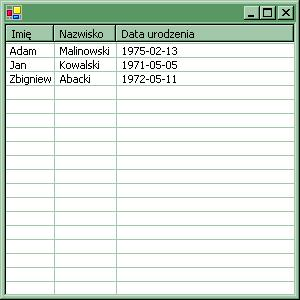
\includegraphics[width=0.50\textwidth]{./pic/swf03}
\caption{ListView potrafi sam sortować elementy umieszczone na liście}
\end{center}
\end{figure}

\begin{scriptsize}
\begin{verbatim}
/* Wiktor Zychla, 2003 */
using System;
using System.Collections;
using System.Drawing;
using System.Windows.Forms;

namespace Example
{
  // klasa do porównywania elementów ListView
  // wg. wskazanej kolumny
  public class MyLVItemSorter : IComparer
  {
    int kolumna; // kolumna wg. której sortujemy

    public MyLVItemSorter( int kolumna )
    {
      this.kolumna = kolumna;
    }

    public int Compare( object o1, object o2 )
    {
      ListViewItem l1 = o1 as ListViewItem;
      ListViewItem l2 = o2 as ListViewItem;

      return string.Compare( l1.SubItems[ kolumna ].Text,
                             l2.SubItems[ kolumna ].Text );
    }
  }

  public class CMainForm : Form
  {   
    ListView lstItems;

    void InitListViewElements()
    {
      string[] sHeaders = new string[] { "Imię", "Nazwisko", "Data urodzenia" };
      ListViewItem li;
     
      // nagłówki 
      lstItems.Columns.Clear();
      foreach ( string s in sHeaders )
        lstItems.Columns.Add( s, 60, HorizontalAlignment.Left ); 
      
      // elementy
      li = lstItems.Items.Add( "Jan" );     
      li.SubItems.Add( "Kowalski" );
      li.SubItems.Add( "1971-05-05" );

      li = lstItems.Items.Add( "Adam" );
      li.SubItems.Add( "Malinowski" );
      li.SubItems.Add( "1975-02-13" );

      li = lstItems.Items.Add( "Zbigniew" );
      li.SubItems.Add( "Abacki" );
      li.SubItems.Add( "1972-05-11" );

      // dopasuj szerokości kolumn
      foreach ( ColumnHeader ch in lstItems.Columns )
        ch.Width = -2;
    }

    // po kliku w kolumnę ListView ustal sortowanie wg. tej kolumny
    void LV_ColumnClick( object sender, ColumnClickEventArgs e )
    {
      lstItems.ListViewItemSorter = new MyLVItemSorter( e.Column );
    }

    public CMainForm()
    {
      lstItems      = new ListView();
      lstItems.Dock = DockStyle.Fill;
      lstItems.FullRowSelect = true;
      lstItems.GridLines = true;
      lstItems.View      = System.Windows.Forms.View.Details;       
      lstItems.ColumnClick += new ColumnClickEventHandler( LV_ColumnClick );
     
      this.Controls.Add( lstItems );

      InitListViewElements(); 
    } 

    public static void Main()
    {
      Application.Run( new CMainForm() );
    }
  }
}
\end{verbatim}
\end{scriptsize}

\subsubsection{TreeView}

Komponent {\bf TreeView} zyskał nowy, obiektowy interfejs, w którym każdy węzeł ma kolekcję {\bf Nodes}, 
przechowującą jego podwęzły. 

Z komponentem tym wiąże się klasyczny problem: jak radzić sobie z wypełnianiem struktury TreeView, jeśli 
powinien on przechowywać bardzo dużo danych? Oczywiście zainicjowanie całego drzewa w konstruktorze
okna macierzystego może nie wchodzić w grę, właśnie z powodu dużej ilości danych.

Problem ten rozwiązuje się zwykle tak, że inicjuje się tylko {\em jeden} poziom drzewa, poziom główny,
dodając przy okazji tym węzłom, które mają przechowywać jakieś podwęzły, tylko {\em jeden}, bardzo specjalny
"pusty" podwęzeł, oznaczony w propercji {\bf Tag} w jakiś określony sposób.

Następnie należy dodać funkcję obsługi zdarzenia {\bf BeforeExpand}, które pojawia się, gdy użytkownik
próbuje "rozwijać" węzeł drzewa przy pomocy symbolu "+" umieszczonego przy węźle. Wewnątrz funkcji obsługi
zdarzenia należy sprawdzić, czy rozwijany węzeł ma tylko jeden podwęzeł i to w dodatku ten specjalnie oznakowany.
Jeśli tak - należy ten podwęzeł usunąć i dobudować kolejny poziom drzewa, znów dodając specjalne
"puste" podwęzły określonym węzłom.

W ten sposób drzewo budowane jest zawsze "na życzenie", przy czym dobudowywany jest zawsze tylko ten poziom
drzewa, który jest akurat potrzebny.

\begin{figure}
\begin{center}
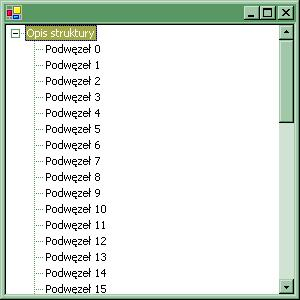
\includegraphics[width=0.50\textwidth]{./pic/swf04}
\caption{TreeView pozwala pokazać zależności między obiektami}
\end{center}
\end{figure}

\begin{scriptsize}
\begin{verbatim}
/* Wiktor Zychla, 2003 */
using System;
using System.Collections;
using System.Drawing;
using System.Windows.Forms;

namespace Example
{
  public class CMainForm : Form
  {   
    TreeView tvItems;

    void InitTVElements()
    {
      TreeNode treeRoot  = new TreeNode( "Opis struktury" );
      treeRoot.ForeColor = Color.Blue;

      TreeNode treeSubNode;
      for ( int i=0; i<45; i++ )
      {
        treeSubNode = new TreeNode( String.Format( "Podwęzeł {0}", i ) );
        treeRoot.Nodes.Add( treeSubNode );
      }   

      tvItems.Nodes.Add( treeRoot );
    } 

    public CMainForm()
    {
      tvItems      = new TreeView();
      tvItems.Dock = DockStyle.Fill;
     
      this.Controls.Add( tvItems );

      InitTVElements();
    } 

    public static void Main()
    {
      Application.Run( new CMainForm() );
    }
  }
}
\end{verbatim}
\end{scriptsize}

\subsection{Rozmieszczanie okien potomnych}

Dobrze zaprojektowany interfejs użytkownika powinien być czytelny i przejrzysty. Jednak przy odrobinie
wprawy i doświadczenia można sobie z tym poradzić. O wiele trudniej jest zaprojektować interfejs tak, aby
pozostawał spójny gdy okno zmienia swoje rozmiary, na przykład gdy jest rozciągane przez użytkownika.

Istnieją dwa możliwe rozwiązania: można albo zabronić zmian rozmiaru okna (przez ustawienie
propercji {\bf FormBorderStyle} na {\bf FormBorderStyle.FixedDialog}) albo reagować na zmianę rozmiaru
okna i dopasowywać rozmiary okien potomnych do rozmiaru okna macierzystego. Oczywiście nie zawsze można
po prostu zabronić zmian rozmiaru okna. Czy w związku z tym .NET wspomaga jakoś proces rozmieszczania
okien potomnych przy zmianie rozmiaru okna macierzystego? Otóż tak. 

\subsubsection{Kotwice i dokowanie}

Najprostszy sposób dopasowywania rozmiarów okna potomnego do rozmiarów okna 
macierzystego to tzw. {\em kotwicowanie}. Wystarczy nadać oknu potomnemu właściwość 
{\em bycia zaczepionym} któregoś z boków okna macierzystego, aby okno potomne zachowywało odległość
od odpowiedniego boku podczas zmiany rozmiarów okna macierzystego.

\begin{scriptsize}
\begin{verbatim}
/* Wiktor Zychla, 2003 */
using System;
using System.Drawing;
using System.Windows.Forms;

namespace Example
{
  public class CMainForm : Form
  {   
    Button b; 

    public CMainForm()
    {
      b          = new Button();
      b.Text     = "Kliknij mnie";
      b.Location = new Point( 40, 40 );
      b.Anchor   = AnchorStyles.Bottom |
                   AnchorStyles.Top    |
                   AnchorStyles.Left   |
                   AnchorStyles.Right;

      this.Controls.Add( b );
    } 

    public static void Main()
    {
      Application.Run( new CMainForm() );
    }
  }
}
\end{verbatim}
\end{scriptsize}

\begin{figure}
\begin{center}
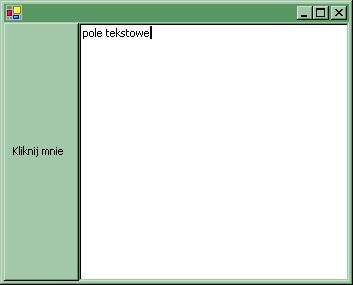
\includegraphics[width=0.50\textwidth]{./pic/swf02}
\caption{Okna potomne zadokowane w obrębie okna macierzystego}
\end{center}
\end{figure}

Okna potomne można również {\em dokować}, czyli przywiązywać na stałe do któregoś z boków lub całego obszaru 
okna macierzystego. Dokowanie jest szczególnie przydatne w przypadku dwóch okien potomnych, bowiem jedno z nich
można zadokować do któregoś z boków, a drugie do całego obszaru okna. Oba okna potomne zajmą wtedy
cały obszar okna macierzystego i będą poprawnie dostosowywać się do zmian jego rozmiaru.

Należy jedynie pamiętać o tym, aby to okno potomne, które powinno wypełniać obszar okna macierzystego
było umieszczone "na wierzchu", czyli nad oknem zadokowanym do któregoś z boków. 

\begin{scriptsize}
\begin{verbatim}
/* Wiktor Zychla, 2003 */
using System;
using System.Drawing;
using System.Windows.Forms;

namespace Example
{
  public class CMainForm : Form
  {   
    Button  b; 
    TextBox t;

    public CMainForm()
    {
      b           = new Button();
      b.Text      = "Kliknij mnie";
      b.Dock      = DockStyle.Left;

      t           = new TextBox();
      t.Multiline = true; 
      t.Dock      = DockStyle.Fill;
      
      this.Controls.Add( t );
      this.Controls.Add( b );
    } 

    public static void Main()
    {
      Application.Run( new CMainForm() );
    }
  }
}
\end{verbatim}
\end{scriptsize}

\subsubsection{Panele}

Sytuacja, w której okno macierzyste ma tylko dwa okna potomne jest niezwykle rzadka. Zastosowanie
pokazanej powyżej metody wydaje się być więc dość ograniczone. Okazuje się jednak, że istnieje specjalny typ
komponentu, {\bf Panel}, który z jednej strony zachowuje się jak okno potomne, bowiem jest 
komponentem umieszczanym wewnątrz jakiegoś okna dialogowego, z drugiej strony zachowuje się jak
okno macierzyste, bowiem ma swoją własną kolekcję okien potomnych, które są kotwicowane i dokowane 
względem obszaru Panela, a nie okna macierzystego.

Można więc używać paneli do podziału okna macierzystego na drobniejsze fragmenty, w obrębie których można
dokonywać odpowiednich ustaleń rozmieszczenia okien potomnych. Panele można zagnieżdżać.

\begin{scriptsize}
\begin{verbatim}
/* Wiktor Zychla, 2003 */
using System;
using System.Drawing;
using System.Windows.Forms;

namespace Example
{
  public class CMainForm : Form
  {   
    Panel   p;
    Button  b1; 
    Button  b2; 
    TextBox t;

    public CMainForm()
    {
      // panel zadokowany do lewej, a w nim dwa przyciski
      p           = new Panel();
      p.Dock      = DockStyle.Left;      

      b1          = new Button();
      b1.Text     = "Kliknij mnie";
      b1.Dock     = DockStyle.Top;

      b2          = new Button();
      b2.Text     = "Kliknij mnie";
      b2.Dock     = DockStyle.Fill;
      
      p.Controls.Add( b2 );
      p.Controls.Add( b1 );

      // pole tekstowe wypełnia obszar okna
      t           = new TextBox();
      t.Multiline = true; 
      t.Dock      = DockStyle.Fill;

      this.Controls.Add( t );
      this.Controls.Add( p );
    } 

    public static void Main()
    {
      Application.Run( new CMainForm() );
    }
  }
}
\end{verbatim}
\end{scriptsize}

\subsubsection{Splittery}

Splittery są elementami graficznymi w postaci poziomych lub pionowych "belek", pozwalających
użytkownikowi zmienić rozmiary okien potomnych. Splitterów używa się tam, gdzie używa się dokowania.

\begin{scriptsize}
\begin{verbatim}
/* Wiktor Zychla, 2003 */
using System;
using System.Drawing;
using System.Windows.Forms;

namespace Example
{
  public class CMainForm : Form
  {   
    Panel   p;   // zawiera b1 i b2  
    Button  b1; 
    Button  b2; 
    TextBox t;

    Splitter s1; // rozdziela b1 i b2
    Splitter s2; // rozdziela p  i t

    public CMainForm()
    {
      // panel zadokowany do lewej, a w nim dwa przyciski
      p           = new Panel();
      p.Dock      = DockStyle.Left;      

      b1          = new Button();
      b1.Text     = "Kliknij mnie";
      b1.Dock     = DockStyle.Top;

      s1          = new Splitter();
      s1.Dock     = DockStyle.Top;

      b2          = new Button();
      b2.Text     = "Kliknij mnie";
      b2.Dock     = DockStyle.Fill;
      
      p.Controls.Add( b2 );
      p.Controls.Add( s1 ); // splitter rozdziela b2 i b1
      p.Controls.Add( b1 );

      // pole tekstowe wypełnia obszar okna
      s2          = new Splitter();
      s2.Dock     = DockStyle.Left;

      t           = new TextBox();
      t.Multiline = true; 
      t.Dock      = DockStyle.Fill;

      this.Controls.Add( t );
      this.Controls.Add( s2 ); // splitter rozdziela t i p
      this.Controls.Add( p );
    } 

    public static void Main()
    {
      Application.Run( new CMainForm() );
    }
  }
}
\end{verbatim}
\end{scriptsize}

\subsection{GDI+}

Tak jak w Win32API istnieją funkcje GDI, tak w świecie .NET istnieje biblioteka GDI+, która
udostępnia obiektowy interfejs do funkcji GDI. 

Używając GDI+ programista musi pamiętać o jednej bardzo ważnej rzeczy. Otóż zainicjowanie obiektu
graficznego, takiego jak pędzel, szczotka, font, obiekt typu {\bf Graphics} itd., spowoduje
utworzenie odpowiedniego elementu w systemie, do którego uchwyt będzie przechowywany wewnątrz obiektu.

Interfejs GDI skonstruowany jest jednak tak, że gdy element graficzny przestaje być potrzebny, powinien
być usunięty, aby system mógł zwolnić zasoby związane z nim. W GDI+ rozwiązano ten problem tak, że
wszystkie obiekty graficzne implementują interfejs {\bf IDisposable}, zaś zasoby systemowe są
zwracane w metodzie {\bf Dispose}. Warto w tym miejscu przypomnieć sobie więc lukier syntaktyczny
ze strony \pageref{disposeSyntaxSugar}, dzięki któremu programista nie musi pamiętać o wywołaniu
metody {\bf Dispose}.

\subsubsection{Obiekt {\bf Graphics}}

W GDI do narysowania czegokolwiek potrzebny był kontekst urządzenia. W GDI+ analogiczną rolę pełni
obiekt typu {\bf Graphics}. 

Obiekt ten jest dostarczany do wszystkich funkcji obsługujących
zdarzenia związane z rysowaniem w parametrze typu {\bf PaintEventArgs} i jest to pewna analogia
do obsługi zdarzenia WM\_PAINT w Win32API.

Obiekt ten może być również utworzony w dowolnej chwili działania aplikacji za pomocą statycznych funkcji
{\bf FromHdc}, {\bf FromHwnd} czy {\bf FromImage}.

Obiekt {\bf Graphics} potrafi wykonać większość operacji związanych z rysowaniem (wymagają wskazania
pędzla jako jednego z parametrów), m.in.:

\begin{itemize}
\item DrawArc
\item DrawBezier
\item DrawEllipse
\item DrawIcon
\item DrawImage
\item DrawLine
\item DrawPath
\item DrawPie
\item DrawRectangle
\item DrawString
\end{itemize}

oraz kilka funkcji związanych z wypełnianiem obszarów (wymagają szczotki jako parametru), m.in:

\begin{itemize}
\item FillEllipse
\item FillPie
\item FillRectangle
\item FillRegion
\end{itemize}

\subsubsection{Kolory}

W każdym miejscu, w którym potrzebne jest określenie koloru, należy skorzystać z obiektu {\bf Color}.
Klasa kolor ma predefiniowane około 140 nazw kolorów, dostępnych jako statyczne propercje, na przykład
{\bf Color.Black}, {\bf Color.AliceBlue}, czy {\bf Color.Red}. Oprócz tego istnieje klasa
{\bf SystemColors}, która udostępnia wartości kolorów przypisanych elementom interfejsu graficznego
Windows. Mamy tu więc m.in. {\bf SystemColors.ActiveBorder}, {\bf SystemColors.Control}, 
czy {\bf SystemColors.WindowText} (w sumie około 25 predefiniowanych kolorów).

W każdej chwili programista może utworzyć własny kolor, opisując jego składowe:

\begin{scriptsize}
\begin{verbatim}
Color c = Color.FromArgb( 40, 50, 60 );
\end{verbatim}
\end{scriptsize}

\subsubsection{Czcionki}

Konstruktor obiektu {\bf Font} pozwala na określenie parametrów czcionki m.in.: 
wielkości, stylu, zestawu znaków. Poniższy przykład jest interesujący również z innego powodu:
czcionka jest tworzona i usuwana, zaś obiekt {\bf Graphics} nie jest usuwany. Jak to wytłumaczyć?

Otóż zauważmy, że obiekt typu {\bf Graphics} jest dostarczony jako parametr w zmiennej typu 
{\bf PaintEventArgs}. Oznacza to, że jest on konstruowany gdzieś indziej. Również gdzieś indziej może
być więc wykorzystywany. Usunięcie go przez {\bf Dispose} mogłoby w szczególnym przypadku objawić się
trudnym do zdiagnozowania błędem.

W przeciwieństwie do obiektu {\bf Graphics}, czcionka jest konstruowana lokalnie i powinna być usunięta
po użyciu. 

\begin{scriptsize}
\begin{verbatim}
/* Wiktor Zychla, 2003 */
using System;
using System.Drawing;
using System.Windows.Forms;

namespace Example
{
  public class CMainForm : Form
  {  
    public CMainForm() {}

    protected override void OnPaint( PaintEventArgs e )
    {
      Graphics g = e.Graphics;

      using ( Font f = new Font( "Courier", 24, FontStyle.Italic ) )
      {
        g.DrawString( "Przykład GDI+", f, Brushes.Black, 0, 0 );
      }
    }

    public static void Main()
    {    
      Application.Run( new CMainForm() );
    }
  }
}
\end{verbatim}
\end{scriptsize}

\subsubsection{Pędzle, szczotki}

GDI+ dostarcza całego zestawu gotowych pędzli i szczotek w obiektach {\bf Pens} i {\bf Brushes}.
W każdym miejscu kodu można z nich skorzystać, a jest to o tyle łatwe, że nazwano je po prostu
nazwami kolorów. Mamy więc na przykład pióro czarne {\bf Pens.Black} czy szczotkę niebieską
{\bf Brushes.Blue}.

Oprócz gotowych piór i szczotek, programista może tworzyć własne. Konstruktor pióra przyjmuje jako parametr
kolor i opcjonalnie grubość pióra:

\begin{scriptsize}
\begin{verbatim}
/* Wiktor Zychla, 2003 */
using System;
using System.Drawing;
using System.Windows.Forms;

namespace Example
{
  public class CMainForm : Form
  {  
    public CMainForm() {}

    protected override void OnPaint( PaintEventArgs e )
    {
      Graphics g = e.Graphics;

      using ( Pen p = new Pen( Color.FromArgb( 40, 50, 130 ), 5 ) )
      {
        g.DrawLine( p, 0, 0, 50, 50 );
      }
    }

    public static void Main()
    {    
      Application.Run( new CMainForm() );
    }
  }
}
\end{verbatim}
\end{scriptsize}

W przypadku szczotek możliwości jest trochę więcej. Istnieje klasa bazowa {\bf Brush}, z której
wyprowadzono klasy umożliwiające tworzenie róznego rodzaju szczotek: {\bf SolidBrush},
{\bf HatchBrush}, {\bf LinearGradientBrush}, {\bf PathGradientBrush} czy {\bf TextureBrush}.

Zobaczmy na przykład jak za pomocą szczotki gradientowej wyposażyć okno w automatycznie odrysowywane
gradientowe tło:

\begin{figure}
\begin{center}
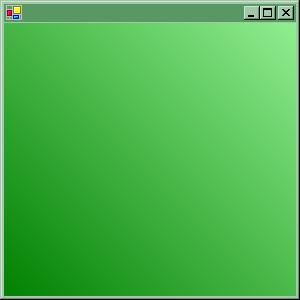
\includegraphics[width=0.50\textwidth]{./pic/swf05}
\caption{Gradientowe tło uzyskane dzięki odpowiedniej szczotce}
\end{center}
\end{figure}

\begin{scriptsize}
\begin{verbatim}
/* Wiktor Zychla, 2003 */
using System;
using System.Drawing;
using System.Drawing.Drawing2D;
using System.Windows.Forms;

namespace Example
{
  public class CMainForm : Form
  {  
    public CMainForm() {}

    protected override void OnPaint( PaintEventArgs e )
    {
      Graphics g = e.Graphics;

      using ( LinearGradientBrush lgb = 
        new LinearGradientBrush( this.ClientRectangle, Color.Green, 
                                 Color.LightGreen, -45f, false ) )
      {
        g.FillRectangle( lgb, this.ClientRectangle );
      }
    }

    protected override void OnResize( EventArgs e )
    {
      Invalidate();
    } 

    public static void Main()
    {    
      Application.Run( new CMainForm() );
    }
  }
}
\end{verbatim}
\end{scriptsize}

\subsubsection{Obrazki}

Tworzenie obrazków możliwe jest dzięki dwóm klasom: {\bf Image} i dziedziczącej z niej {\bf Bitmap}.
Obrazek może być utworzony dynamiczne bądź załadowany z pliku ({\bf Image.FromFile}). 
Obrazek w pamięci można poddać różnym operacjom, można nawet utworzyć obiekt {\bf Graphics} dzięki funkcji
{\bf Graphics.FromImage} i rysować na powierzchni obrazka za pomocą funkcji z GDI+.

Gotowy obrazek można zapisać za pomocą metody {\bf Save}, wybierając przy okazji jeden z dostępnych formatów m.in.
GIF, BMP, PNG, JPG.

Zawartość obrazka można dzięki funkcji {\bf DrawImage} obiektu {\bf Graphics} narysować w kontekście, na który
wskazuje obiekt {\bf Graphics} lub umieścić w komponencie typu {\bf PictureBox}, który może być umieszczony
w oknie. Komponent {\bf PictureBox} sam dba o automatycznie odświeżanie swojej zawartości, programista nie musi
więc odrysowywać zawartości obrazka gdy okno wymaga odświeżenia.

\subsubsection{Podwójne buforowanie}

GDI+ udostępnia możliwość automatycznego podwójnego buforowania wyświetlanej grafiki. Dzięki
temu obraz rysowany jest na niewidocznej stronie graficznej i jest błyskawicznie przenoszony na
powierzchnię okna. Podwójne buforowanie umożliwia całkowite wyeliminowanie efektu "migania" obrazu
podczas rysowania. 

Aktywowanie podwójnego bufowania wymaga jedynie 3 lini kodu w konstruktorze okna:

\begin{scriptsize}
\begin{verbatim}
/* Wiktor Zychla, 2003 */
this.SetStyle(ControlStyles.UserPaint, true);
this.SetStyle(ControlStyles.AllPaintingInWmPaint, true);
this.SetStyle(ControlStyles.DoubleBuffer, true);
\end{verbatim}
\end{scriptsize}

\subsection{Zegary}

Oprogramowanie zegarów jest bardzo proste, ponieważ wystarczy utworzyć obiekt typu {\bf Timer}, 
przypiąć funkcję do listy słuchaczy zdarzenia {\bf Tick} i ustalić interwał czasu między kolejnymi 
zgłoszeniami zdarzenia.

\begin{figure}
\begin{center}
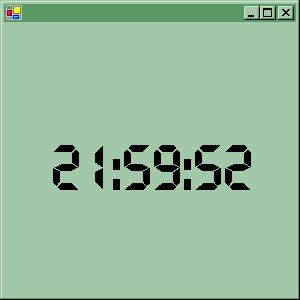
\includegraphics[width=0.50\textwidth]{./pic/swf01}
\caption{Zegarek w C\# z podwójnym buforowaniem grafiki}
\end{center}
\end{figure}

\label{kodZegarek}

\begin{scriptsize}
\begin{verbatim}
/* Wiktor Zychla, 2003 */
using System;
using System.Drawing;
using System.Windows.Forms;

namespace Example
{
  public class CMainForm : Form
  {   
    Timer timer;    

    public CMainForm()
    {
      timer          = new Timer();
      timer.Tick    += new EventHandler( Timer_Tick );
      timer.Interval = 50;
      timer.Start();

      this.SetStyle(ControlStyles.UserPaint, true);
      this.SetStyle(ControlStyles.AllPaintingInWmPaint, true);
      this.SetStyle(ControlStyles.DoubleBuffer, true);
    } 

    void Timer_Tick( object sender, EventArgs e )
    {              
      this.Invalidate();
    }

    protected override void OnPaint( PaintEventArgs e )
    {
      Graphics g = e.Graphics;
      using ( Font f = new Font( "LED", 48 ) )
      {
        StringFormat sf  = new StringFormat();
        sf.Alignment     = StringAlignment.Center;
        sf.LineAlignment = StringAlignment.Center;

        g.Clear( SystemColors.Control );
        g.DrawString( DateTime.Now.ToLongTimeString(), f, Brushes.Black, 
                      this.Width / 2, this.Height / 2, sf );
      }
    }

    public static void Main()
    {
      Application.Run( new CMainForm() );
    }
  }
}
\end{verbatim}
\end{scriptsize}


\subsection{Menu}

\subsubsection{Tworzenie menu}

Tworzenie menu możliwe jest dzięki dwóm typom danych:
\begin{description}
\item [MainMenu] który służy do tworzenia menu dla okna dialogowego
\item [ContextMenu] który służy do tworzenia menu kontekstowych dla okien
\end{description}

\begin{scriptsize}
\begin{verbatim}
/* Wiktor Zychla, 2003 */
using System;
using System.Drawing;
using System.Windows.Forms;

namespace Example
{
  public class CMainForm : Form
  {   
    TextBox tb; 

    void InitMenus()
    {
      // MainMenu
      MainMenu mainMenu = new MainMenu();

      MenuItem mPlik = new MenuItem( "Plik" );
      MenuItem mPlikZakoncz = new MenuItem( "Zakończ" );
      mPlikZakoncz.Click += new EventHandler( mPlikZakoncz_Click );

      mPlik.MenuItems.Add( mPlikZakoncz );
      mainMenu.MenuItems.Add( mPlik );

      this.Menu = mainMenu; 

      // ContextMenu
      ContextMenu cMenu = new ContextMenu();
      MenuItem mZakoncz = new MenuItem( "Zakończ" );
      cMenu.MenuItems.Add( mZakoncz );
      
      this.tb.ContextMenu = cMenu;
    }

    void mPlikZakoncz_Click( object sender, EventArgs e )
    { 
      this.Close();
    } 

    public CMainForm()
    {
      tb = new TextBox();
      this.Controls.Add( tb );

      InitMenus();
    } 

    public static void Main()
    {
      Application.Run( new CMainForm() );
    }
  }
}
\end{verbatim}
\end{scriptsize}

Obiekt typu {\bf ContextMenu}, reprezentujący menu kontekstowe, ma jeszcze jedną interesującą
właściwość. Otóż ma on metodę {\bf Show}, która po prostu pokazuje menu kontekstowe przy
wskazanym oknie potomnym. Jest to bardzo wygodne wtedy, kiedy menu kontekstowe powinno zostać
ujawnione w jakiejś nietypowej sytuacji. 

Wyobraźmy sobie na przykład scenariusz, w którym każdemu elementowi drzewa {\bf TreeView} powinno odpowiadać
jakieś inne menu kontekstowe, zależne od tego, co zawiera wskazany element. Zamiast przywiązywać jakieś
konkretne menu kontekstowe do obiektu {\bf TreeView}, programista może po prostu przechwycić 
zdarzenie kliknięcia myszą w węzeł drzewa, sprawdzić czy kliknięto prawy klawisz myszy i dopiero
wtedy wykorzystać metodę {\bf Show} do pokazania odpowiedniego menu kontekstowego.

\subsubsection{Własne funkcje rysowania menu}

Wygląd menu można uatrakcyjnić dzięki możliwości określenia własnych funkcji odpowiedzialnych
za rysowanie elementów menu. Programista musi jedynie dodać funkcje obsługi zdarzeń {\bf DrawItem}, 
odpowiedzialnej za rysowanie i {\bf MeasureItem}, odpowiedzialnej za określanie obszaru zajmowanego przez
element menu\footnote{Kilku innym komponentom wizualnym również można zmieniać wygląd w taki sposób.}.

W poniższym przykładzie zmieniamy sposób rysowania tylko tych pozycji menu, które widoczne są
na pasku menu w oknie. W analogiczny sposób można jednak określić sposób rysowania pozycji rozwijalnych,
dodając na przykład możliwość rysowania ikon obok pozycji menu itp.

\begin{scriptsize}
\begin{verbatim}
/* Wiktor Zychla, 2003 */
using System;
using System.Drawing;
using System.Windows.Forms;

namespace WinForms_Dodatki
{
  public class C_XMainMenu : System.Windows.Forms.MainMenu 
  {
    private void topMenu_DrawItem(object sender, 
                                  System.Windows.Forms.DrawItemEventArgs e)
    {
      Rectangle mRect  = 
        new Rectangle(e.Bounds.X, e.Bounds.Y, e.Bounds.Width, e.Bounds.Height);
      Rectangle mRect2 = 
        new Rectangle(e.Bounds.X, e.Bounds.Y, e.Bounds.Width+1, e.Bounds.Height+1);

      if ( (e.State & DrawItemState.Selected) != 0 )  
      {
        e.Graphics.FillRectangle( new SolidBrush( SystemColors.Control ), mRect );
        e.Graphics.DrawRectangle( 
          new Pen( new SolidBrush( SystemColors.ControlDark ), 1 ), mRect );
      }
      else
      if ( (e.State & DrawItemState.HotLight) != 0 ) 
      {
        e.Graphics.FillRectangle( new SolidBrush( SystemColors.ControlLightLight ), mRect );
        e.Graphics.DrawRectangle( 
          new Pen( new SolidBrush( SystemColors.ControlDark ), 1 ), mRect );
      }
      else
      {
        e.Graphics.FillRectangle( new SolidBrush(SystemColors.Control), mRect2 );
      }
						
      MenuItem     mItem   = (MenuItem)sender;
      Font         mFont   = new Font( "MS Sans Serif", 10 );
      StringFormat sFormat = new StringFormat();
			
      sFormat.Alignment     = StringAlignment.Center;
      sFormat.LineAlignment = StringAlignment.Center;

      e.Graphics.DrawString(mItem.Text, mFont, new SolidBrush(Color.Black), mRect, sFormat );

      mFont.Dispose();
    }

    private void topMenu_MeasureItem(object sender, 
                            System.Windows.Forms.MeasureItemEventArgs e)
    {
      MenuItem     mItem = (MenuItem)sender;
      Font         mFont = new Font( "MS Sans Serif", 10 );

      SizeF sizeF  = e.Graphics.MeasureString( mItem.Text, mFont );			
      e.ItemWidth  = (int)sizeF.Width;

      mFont.Dispose();
    }

    public C_XMainMenu( Menu mMenu ) 
    {
      foreach ( MenuItem mItem in mMenu.MenuItems )
      {				
        MenuItem newMenuItem = mItem.CloneMenu();
				
        ApplyMenuProperties ( newMenuItem );
        this.MenuItems.Add ( newMenuItem );
      }			
    }
		
    private void ApplyMenuProperties( MenuItem mItem )
    {
      if ( IsTopMenu( mItem ) )
      {
        mItem.OwnerDraw = true;
        mItem.DrawItem += 
	  new System.Windows.Forms.DrawItemEventHandler(this.topMenu_DrawItem);
        mItem.MeasureItem += 
	  new System.Windows.Forms.MeasureItemEventHandler(this.topMenu_MeasureItem);				
      }

      foreach ( MenuItem subMenu in mItem.MenuItems )
        ApplyMenuProperties( subMenu );
    }

    private static bool IsTopMenu( MenuItem mItem )
    {
      if ( mItem.Parent == null ) return true;
      return mItem.Parent == mItem.GetMainMenu();
    }
  }
}
\end{verbatim}
\end{scriptsize}

Klasa {\bf C\_XMainMenu} określona jest tak, że w kodzie inicjującym menu należy po prostu napisać:

\begin{scriptsize}
\begin{verbatim}
MainMenu mainMenu;
...
C_XMainMenu cxMainMenu = new C_XMainMenu( mainMenu );
this.Menu = cxMainMenu; 
\end{verbatim}
\end{scriptsize}

\subsection{Schowek}

Dostęp do schowka systemowego możliwy jest dzięki obiektowi {\bf Clipboard}. W schowku można
umieścić dowolny obiekt lub sprawdzić czy znajduje się tam obiekt określonego typu.

Poniższy przykład umieszcza w schowku napis, a następnie wydobywa go stamtąd. Dane przekazane
do schowka w ten sposób są dostępne dla wszystkich aplikacji w systemie, podobnie dane
pobierane ze schowka mogą pochodzić z dowolnej aplikacji w systemie.

\begin{scriptsize}
\begin{verbatim}
/* Wiktor Zychla, 2003 */
using System;
using System.Drawing;
using System.Windows.Forms;

namespace Example
{
  public class CMainForm : Form
  {  
    public CMainForm() 
    {
      // umieść dane w schowku
      Clipboard.SetDataObject( "Tekst przesyłany do schowka", true );

      // wydobądź dane ze schowka
      IDataObject ido = Clipboard.GetDataObject();
      if ( ido.GetDataPresent( typeof( string ) ) )
      {
        string s = ido.GetData( typeof( string ) ) as string;
        MessageBox.Show( s );
      }
    }

    public static void Main()
    {    
      Application.Run( new CMainForm() );
    }
  }
}
\end{verbatim}
\end{scriptsize}


\subsection{Drag \& drop}

\subsection{Tworzenie własnych komponentów}

Jedną z najciekawszych możliwości nowoczesnych technologii informatycznych jest możliwość definiowania
własnych komponentów wizualnych. Kiedy nie było jeszcze technologii .NET własne komponenty można było
tworzyć w technologii COM, używając do tego Visual Basica lub C++. 

Możliwości .NET jeszcze bardziej ułatwiają cały ten proces. Tak naprawdę wystarczy utworzyć klasę
dziedziczącą z {\bf UserControl} i już może ona funkcjonować jako komponent wizualny. Taki własny
komponent może na przykład składać się z dowolnej ilości już istniejących komponentów i automatyzować
pewne zależności między nimi, może też tworzyć całkowicie nowe możliwości interfejsowe.

Do czego może przydawać się możliwość tworzenia własnych komponentów? 

Wyobraźmy sobie na przykład, że
standardowy komponent {\bf ComboBox} chcielibyśmy wyposażyć w automatyczne dopasowywanie elementu na liście
do tekstu wpisywanego przez użytkownika. Zwykły ComboBox tego nie potrafi, ale można utworzyć własny
komponent i dodać reakcje na odpowiednie zdarzenia, by uzyskać porządaną funkcjonalność. Można taki problem
rozwiązać bez tworzenia nowego komponentu, tyle że gdyby chcieć użyć takiego ComboBoxa więcej niż raz,
utworzenie jednego komponentu wielokrotnego użycia, po prostu ogromnie upraszcza życie programisty.

Wyobraźmy sobie również, że chcielibyśmy mieć zupełnie nowy komponent wizualny, siatkę, z możliwością
dodawania wierszy i kolumn i to taką, żeby każda komórka mogła mieć inny kolor, czcionkę wyrównanie czy
orientację tekstu. Takiego komponentu standardowo w bibliotece komponentów .NET nie ma.
Możnaby jednak utworzyć własny komponent, dodać mu jakieś struktury danych do przechowywania danych,
dodać jakieś propercje, metody i zdarzenia, tak aby można było sterować takim komponentem z poziomu kodu
konkretnego okna, w którym byłby on osadzony, a następnie przeciążyć całkowicie metodę {\bf OnPaint}, dzięki
czemu wizualna zawartość komponentu mogłaby być tworzona całkowicie dowolnie, bez żadnego związku z już
istniejącymi komponentami.

\subsubsection{Najprostszy komponent}

Zaczniemy od bardzo prostego przykładu komponentu, który będzie tylko
wypisywał tekst w swoim obszarze. Komponent taki jset oknem leżącym gdzieś w jakimś innym oknie.
Wewnątrz kodu może więc dowiedzieć się jakie są jego bieżące rozmiary za pomocą propercji
{\bf Width} i {\bf Height}. Również propercje takie jak {\bf Font}, {\bf Text}, {\bf BackColor} czy
{\bf ForeColor} są, jako dziedziczone z klasy {\bf UserControl}, dostępne dla klienta komponentu.

Klient komponentu (czyli kod, który korzysta z tego komponentu) traktuje więc nowo zaprojektowany komponent
jak każdy inny - może ustalać rozmiary komponentu, jego kotwicowanie czy dokowanie oraz używać 
wszystkich potrzebnnych propercji, zdarzeń i metod (tak prosty komponent nie ma żadnych sensownych
składowych poza tymi dziedziczonymi z {\bf UserControl}).

W środowisku wizualnym tak zaprojektowany komponent po umieszczeniu w bibliotece obiektowej
(takie jest ograniczenie na przykład VisualStudio) mógłby być umieszczony na przyborniku z komponentami i
umieszczany na oknach jak każdy inny komponent z przybornika!

\begin{figure}
\begin{center}
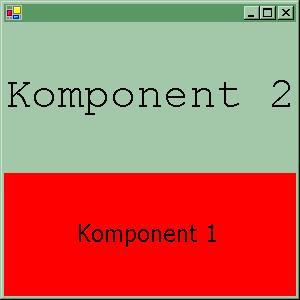
\includegraphics[width=0.50\textwidth]{./pic/swf06}
\caption{Najprostszy komponent}
\end{center}
\end{figure}

\begin{scriptsize}
\begin{verbatim}
/* Wiktor Zychla, 2003 */
using System;
using System.Drawing;
using System.Windows.Forms;

namespace Example
{
  public class CKomponent : UserControl
  {
    public CKomponent() {}

    protected override void OnPaint( PaintEventArgs e )
    {
      StringFormat sf  = new StringFormat();
      sf.Alignment     = StringAlignment.Center;
      sf.LineAlignment = StringAlignment.Center;

      e.Graphics.Clear( this.BackColor );
      e.Graphics.DrawString( this.Text, this.Font, Brushes.Black, 
                             this.Width / 2, this.Height / 2, sf );
    }

    protected override void OnResize( EventArgs e )
    {
      Invalidate();
    }
  }

  public class CMainForm : Form
  {  
    CKomponent ck1, ck2;

    public CMainForm() 
    {
      ck1      = new CKomponent();
      ck1.Text = "Komponent 1";
      ck1.BackColor = Color.Red;
      ck1.Font = new Font( "Tahoma", 18 );
      ck1.Size = new Size( 50, 50 );
      ck1.Dock = DockStyle.Fill;

      ck2      = new CKomponent();
      ck2.Text = "Komponent 2";
      ck2.Font = new Font( "Courier", 32 );
      ck2.Dock = DockStyle.Top;

      this.Controls.AddRange( new Control[] { ck1, ck2 } );
    }

    public static void Main()
    {    
      Application.Run( new CMainForm() );
    }
  }
}
\end{verbatim}
\end{scriptsize}

\subsubsection{Komponent złożony}

Komponent może zawierać w sobie dowolną ilość innych komponentów i wewnątrz swojego kodu
przechwytywać ich zdarzenia.

\begin{scriptsize}
\begin{verbatim}
/* Wiktor Zychla, 2003 */
using System;
using System.Drawing;
using System.Windows.Forms;

namespace Example
{
  public class CKomponent : UserControl
  {
    Button b1, b2;

    public CKomponent() 
    {
      b1      = new Button();
      b1.Text = "1";
      b1.Dock = DockStyle.Fill;
      b1.Click += new EventHandler( bt_Click );

      b2      = new Button();
      b2.Text = "2";
      b2.Size = new Size( 40, 40 );
      b2.Dock = DockStyle.Right;
      b2.Click += new EventHandler( bt_Click );

      this.Controls.AddRange( new Control[] { b1, b2 } );
    }

    public void bt_Click( object sender, EventArgs e )
    {
      MessageBox.Show( ((Control)sender).Text );
    } 
  }

  public class CMainForm : Form
  {  
    CKomponent ck1, ck2;

    public CMainForm() 
    {
      ck1      = new CKomponent();
      ck1.Text = "Komponent 1";
      ck1.BackColor = Color.Red;
      ck1.Font = new Font( "Tahoma", 8 );
      ck1.Size = new Size( 50, 50 );
      ck1.Dock = DockStyle.Fill;

      ck2      = new CKomponent();
      ck2.Text = "Komponent 2";
      ck2.Font = new Font( "Courier", 12 );
      ck2.Dock = DockStyle.Top;

      this.Controls.AddRange( new Control[] { ck1, ck2 } );
    }

    public static void Main()
    {    
      Application.Run( new CMainForm() );
    }
  }
}
\end{verbatim}
\end{scriptsize}

\subsubsection{Definiowanie własnych zdarzeń}

Zestaw zdarzeń udostępnianych przez komponenty również może być rozbudowany. Wyobraźmy sobie, że
chcielibyśmy mieć komponent, który zawierałby {\bf ComboBox} i mały przycisk z napisem "+" z boku.
Chcielibyśmy, aby użytkownik mógł użyć tego przycisku do dodawania nowych elementów do ComboBoxa.
Z punktu widzenia logiki tego komponentu zdarzenie oznaczające chęć dodania nowego elementu mogłoby
jednak pojawiać się również wtedy, kiedy użytkownik wpisałby w pole tekstowe {\bf ComboBoxa} jakiś tekst spoza
tekstów dostępnych na liście. To już aż dwa przypadki, kiedy takie zdarzenie mogłoby się pojawić.

Możemy więc zaprojektować nowe zdarzenie. Nazwiemy je {\bf AddNewText}. Być może w toku prac
okazałobysię, że zdarzenie takie powinno mieć jakieś dodatkowe parametry. Zaprojektowalibyśmy wtedy
nową klasę, {\bf AddNewTextEventArgs} i zmodyfikowalibyśmy deklarację zdarzenia. Należałoby jedynie
pamiętać o zachowaniu konwencji: odpowiedni delegat powinien mieć dwa parametry, z czego pierwszy
powinien wskazywać na źródło zdarzenia, drugi powinien dziedziczyć z klasy {\bf EventArgs},
rozszerzając ją o dodatkowe parametry zdarzenia.

Zauważmy, że kod klienta korzysta z tego zdarzenia tak samo jak z każdego zdarzenia. Z punktu widzenia
kodu nie ma różnicy między naszym nowym zdarzeniem, a już istniejącymi zdarzeniami.

\begin{scriptsize}
\begin{verbatim}
/* Wiktor Zychla, 2003 */
using System;
using System.Drawing;
using System.Windows.Forms;

namespace Example
{  
  public class CComboBox : UserControl
  {
    ComboBox cb;
    Button   bt;

    // własne zdarzenie definiowane przez komponent
    public event EventHandler AddNewText;

    public CComboBox() 
    {
      cb      = new ComboBox(); 
      cb.Dock = DockStyle.Fill;
      
      bt      = new Button();
      bt.FlatStyle = FlatStyle.Popup;
      bt.Text = "+";
      bt.Dock = DockStyle.Right; 
      bt.Click += new EventHandler( bt_Click );

      this.Controls.AddRange( new Control[] { cb, bt } );
    }

    protected override void OnResize( EventArgs e )
    {
      bt.Size = new Size( this.Height, this.Height );           
    }    

    // przechwyć klik w przycisk i na zewnątrz wystaw jako AddNewText
    void bt_Click( object sender, EventArgs e )
    {
      // sprawdź czy są jacyś słuchacze     
      if ( AddNewText != null )
        AddNewText( this, new EventArgs() );
    }
  }

  public class CMainForm : Form
  {  
    CComboBox cb1;

    public CMainForm() 
    {
      cb1      = new CComboBox();
      cb1.Size = new Size( 150, 20 );

      cb1.AddNewText += new EventHandler( cb_AddNewText );

      this.Controls.Add( cb1 );
    }

    void cb_AddNewText( object sender, EventArgs e )
    {
      MessageBox.Show( "Zgłoszono zdarzenie AddNewText!" );
    }

    public static void Main()
    {    
      Application.Run( new CMainForm() );
    }
  }
}
\end{verbatim}
\end{scriptsize}

\subsection{Typowe okna dialogowe}

\subsubsection{Okna wyboru plików}

Standardowo, programista ma do dyspozycji okno wyboru pliku do otwarcia i zamknięcia
({\bf OpenFileDialog} i {\bf SaveFileSialog}). Oba działają
bardzo podobnie - po ustaleniu właściwości należy wywołać metodę do pokazania okna i
przechwycić rezultat, wskazujący na to czy przypadkiem użytkownik nie anulował okna. 
Lista wybranych plików dostępna jest dzięki propercji {\bf FileName[s]}.

\begin{scriptsize}
\begin{verbatim}
/* Wiktor Zychla, 2003 */
using System;
using System.Drawing;
using System.Windows.Forms;

namespace Example
{
  public class CMainForm : Form
  {  
    public CMainForm() 
    {
      OpenFileDialog of   = new OpenFileDialog();
      of.InitialDirectory = 
        Environment.GetFolderPath( Environment.SpecialFolder.ProgramFiles );
      of.Title            = "Wybierz plik do otwarcia...";
      of.Filter           = "Moje pliki (*.xyz)|*.xyz|"+
                            "Wszystkie pliki (*.*)|*.*";
      of.Multiselect      = true;

      DialogResult res = of.ShowDialog();
      if ( res == DialogResult.OK )
        foreach ( string fileName in of.FileNames )
          MessageBox.Show( "Wybrano plik " + fileName );
    }

    public static void Main()
    {    
      Application.Run( new CMainForm() );
    }
  }
}
\end{verbatim}
\end{scriptsize}

\subsubsection{Okno wyboru czcionki}

\begin{scriptsize}
\begin{verbatim}
/* Wiktor Zychla, 2003 */
using System;
using System.Drawing;
using System.Windows.Forms;

namespace Example
{
  public class CMainForm : Form
  {  
    public CMainForm() 
    {
      FontDialog fd    = new FontDialog();
      fd.ShowColor     = true;
      fd.ShowEffects   = true;

      DialogResult res = fd.ShowDialog();
      if ( res == DialogResult.OK )
        MessageBox.Show( "Wybrano czcionkę: " + fd.Font.ToString() );
    }

    public static void Main()
    {    
      Application.Run( new CMainForm() );
    }
  }
}
\end{verbatim}
\end{scriptsize}

\subsubsection{Okno wyboru koloru}

\begin{scriptsize}
\begin{verbatim}
/* Wiktor Zychla, 2003 */
using System;
using System.Drawing;
using System.Windows.Forms;

namespace Example
{
  public class CMainForm : Form
  {  
    public CMainForm() 
    {
      ColorDialog cd   = new ColorDialog();
      cd.AllowFullOpen = true;

      DialogResult res = cd.ShowDialog();
      if ( res == DialogResult.OK )
        MessageBox.Show( "Wybrano kolor: " + cd.Color.ToString() );
    }

    public static void Main()
    {    
      Application.Run( new CMainForm() );
    }
  }
}
\end{verbatim}
\end{scriptsize}
